\documentclass[12pt]{article}

\usepackage[margin=2cm]{geometry}
\usepackage{amsmath}
\usepackage{multicol}
\usepackage{nopageno}
\usepackage{SIunits}
\usepackage{graphicx}
\usepackage{enumerate}
\usepackage{enumitem}
%\usepackage{mathabx}
\usepackage{wasysym}


% for making bond drawings
\usepackage{chemfig}
% Global bond settings
\setchemfig{
  atom sep=18pt,               % fixed bond length
  double bond sep=2pt,       % spacing between the two bars
  bond style={line width=0.8pt}
}


% for centering figures on page while in an enumerated/itemized list:
\usepackage{changepage} % in the preamble
\makeatletter
\newenvironment{centerinpage}
  {%
    \par\noindent
    \hspace*{-\@totalleftmargin}% back to page margin (covers all nested list indents)
    \begin{minipage}{\textwidth}% fixed to page width (ignores widened \linewidth)
      \centering
  }
  {%
    \end{minipage}\par
  }
\makeatother

%%%%%%%%%%%%%%%%%%%%%%%%%%%%%%%%%%%%%%%%%%%%%%%%%%%%%
% For putting links in the document (both to sections and hyperlinks)
\usepackage{hyperref}
\usepackage{url}
\hypersetup{
    colorlinks=true,     % false: boxed links; true: colored links
    linkcolor=red,       % color of internal links
    citecolor=blue,      % color of links to bibliography
    filecolor=blue,      % color of file links
    urlcolor=blue        % color of external links
}
% below, use \url{http://www.nytimes.com} (they will be urlcolor)
%%%%%%%%%%%%%%%%%%%%%%%%%%%%%%%%%%%%%%%%%%%%%%%%%%%%%


%%%%%%%%%%%%%%%%%%%%%%%%%%%%%%%%%%%%%%%%%%%%%%%%%%%%%
% for the events page boxes

% boxed regions
\usepackage{tcolorbox}
\tcbuselibrary{skins,breakable}

% fonts & spacing
\usepackage{lmodern}
\usepackage{microtype}
\usepackage{calc}


% small helper macros (adjust these)
\newcommand{\boxheight}{4.2cm}   % height for each event box
\newcommand{\boxfont}{\scriptsize} % change to \tiny or \footnotesize as desired
\newcommand{\linelen}{0.95\linewidth} % timeline line length

%%%%%%%%%%%%%%%%%%%%%%%%%%%%%%%%%%%%%%%%%%%%%%%%%%%%%
\newcommand{\rmd}{\ensuremath{{\rm d}}}
%\newcommand{\vv}[1]{\ensuremath{\vec{#1}}}
\newcommand{\vv}[1]{\ensuremath{\mathbf{#1}}}
\newcommand{\ee}[1]{\ensuremath{\mathbf{e}_{#1}}}
%%%%%%%%%%%%%%%%%%%%%%%%%%%%%%%%%%%%%%%%%%%%%%%%%%%%%



\begin{document}

\begin{center}
{\Large Climate Sensitivity}
\end{center}
%%%%%%%%%%%%%%%%%%%%%%%%%%%%%%%%%%%%%%%%%%%%%%%%
%%%%%%%%%%%%%      overview         %%%%%%%%%%%%%%%%%%%%%
%%%%%%%%%%%%%%%%%%%%%%%%%%%%%%%%%%%%%%%%%%%%%%%%

The term {\bf climate sensitivity} is used both as a technical term meaning {\em the Earth's equilibrium temperature increase due to a doubling in carbon dioxide concentration}\footnote{I will use the phrase {\em carbon dioxide concentration} to mean the mole fraction of carbon dioxide in the air, which is just the fraction of all molecules in the air --- regardless of the molecule type,  size, or mass --- that are $\text{CO}_2$. This \href{https://gml.noaa.gov/ccgg/trends/}{value is presently $\unit{425}{ppm}$} $ = \frac{425}{1000000} = 0.000425 = 0.0425\%$, meaning that 425 out of every million molecules of air are carbon dioxide. Nitrogen and Oxygen are the primary atmospheric gases with concentrations of 80\% and 20\%, respectively, so almost 800,000 and 200,000 per million particles are those.  Methane, another greenhouse gas, has a \href{https://gml.noaa.gov/ccgg/trends_ch4/}{current concentration of \unit{1930}{ppb}} (parts per billion), so two out of every million molecules of air, or  $0.00019$\%.}, and as a general term to mean {\em the effect of increasing greenhouse gas concentrations on temperature}. Today we will look closely at the blackbody curve of the Earth's infrared emission (due to its average surface temperature of approximately $15\degree \text{C} = \unit{288}{\kelvin}$), and the $\text{CO}_2$ absorption lines in that spectrum, to understand (i) how greenhouse gas absorption causes temperature increase, and (ii) what we should expect that relationship to look like.

%
%\newpage
%%%%%%%%%%%%%%%%%%%%%%%%%%%%%%%%%%%%%%%%%%%%%%%%
%%%%%%%%%%%%%      questions         %%%%%%%%%%%%%%%%%%%%%
%%%%%%%%%%%%%%%%%%%%%%%%%%%%%%%%%%%%%%%%%%%%%%%%

\begin{enumerate}

\item  Let's start by carefully examining simulated blackbody curves of the Earth surface's emission to space as it would be\footnote{In fact we do measure the Earth's spectrum from space, using insturments on \href{https://en.wikipedia.org/wiki/Atmospheric_infrared_sounder}{NASA's  ``Aqua''  satellite using the AIRS and CERES instruments}.} observed from space.
	%
	\begin{enumerate}
	\item The blackbody curves shown in Figure \ref{fig:archer-earth-bb} are plotted as a function of wavenumber.  Convert our familiar wavelength for the carbon dioxide bending transition ($\lambda = \unit{15}{\micro\meter}$), which takes the biggest ``bite'' out of the Earth's infrared blackbody spectrum, into wavenumber and frequency.  Use the following equations to do so, expressing your final result in units of $\text{cm}^{-1}$ for wavenumber and in units of $\text{THz} = \unit{10^{12}}{\hertz}$ for frequency:
		%
		\begin{equation*}
		f \, \lambda = c \quad \quad \text{and} \quad \quad  \bar{\nu} = \frac{1}{\lambda}
		\end{equation*}
		%
	where $c = {3\times10^8}{\meter/\second}$ is the speed of light, $f$ is the variable for frequency, $\tilde{\nu}$ (``nu tilda'') is the variable most often used for wavenumber. Does your answer for wavenumber make sense based on the absorption lines seen in Figure \ref{fig:archer-earth-bb}?  Does your answer for frequency make sense based on the graphs shown in Figure \ref{fig:andrews-co2-absorption}? Why or why not?
	\item Looking at the graph in the top of Figure \ref{fig:archer-earth-bb}, what do you estimate to be the temperature of the emitted light?  [In the regions where there are no bites, which blackbody curve would best fit?]
	\item Why does the $\text{CO}_2$ absorption line have a flat base?  
	\item Why does the Ozone absorption line have a little peak in the middle? (Notice in the actual data plotted in Figure \ref{fig:archer-earth-bb} (bottom) that the carbon dioxide also has such a peak.)
	\item Approximate the $T=\unit{240}{\kelvin}$ blackbody curve with a triangle by drawing it over the graph (the base of the triangle should lie on the horizontal axis).  Calculate the area of this triangle using the values and units shown on the axes.  What units does it have? What do we call this quantity? Does the number you found make sense based on our prior work?
	\end{enumerate}
	
\newpage
	
\item Now let's try to understand how $\text{CO}_2$ absorption lines lead to an increased overall temperature of the Earth.
	%
	\begin{enumerate}
	\item Figure \ref{fig:archer-earth-bb-w-diff-CO2} shows simulated blackbody curves for the Earth's infrared emission, with different amounts of atmospheric $\text{CO}_2$.  Describe generally how the absorption line changes as carbon dioxide is added to the atmosphere.
	\item When does the $\text{CO}_2$ absorption line ``saturate'' and what does that mean?
	\item On graph paper, draw an ``approximate'' blackbody curve as a (dashed-line) isosceles triangle with the following characteristics: base points at \unit{5}{\micro\meter} and \unit{25}{\micro\meter}; a peak of \unit{23.8}{\watt/\meter^2/\micro\meter}. What is its area under the curve?
	\item Make a carbon dioxide ``absorption line'' in your curve centered at  \unit{15}{\micro\meter}.  Give it a depth that shows ``saturation'' (not all the way down to zero) and try to give it a width so that it ``eats'' $\frac{1}{3}$ to $\frac{1}{2}$ of the original area.  What is the area of your triangle with the absorption line removed?
	\item Try to draw another isosceles triangle (with same base) that also has an absorption line of the same width and (fractional depth), but has total area equal to the original (un-eaten) triangle.  
	\end{enumerate}
	
	

\end{enumerate}

\newpage

%%%%%%%%%%%%%%%%%%%%%%%%%%%%%%
%\mbox{}
%\newpage
%%%%%%%%%%%%%%%%%%%%%%%%%%%%%%

%%%%%%%%%%%%%%%%%%%%%%%%%%%%%%%%%%%%%%%%%%%%%%%%%%%%
%%%%%%%%%%               milankovitch wikimedai            %%%%%%%%%%%%%
%%%%%%%%%%%%%%%%%%%%%%%%%%%%%%%%%%%%%%%%%%%%%%%%%%%%

\begin{figure}
\centering
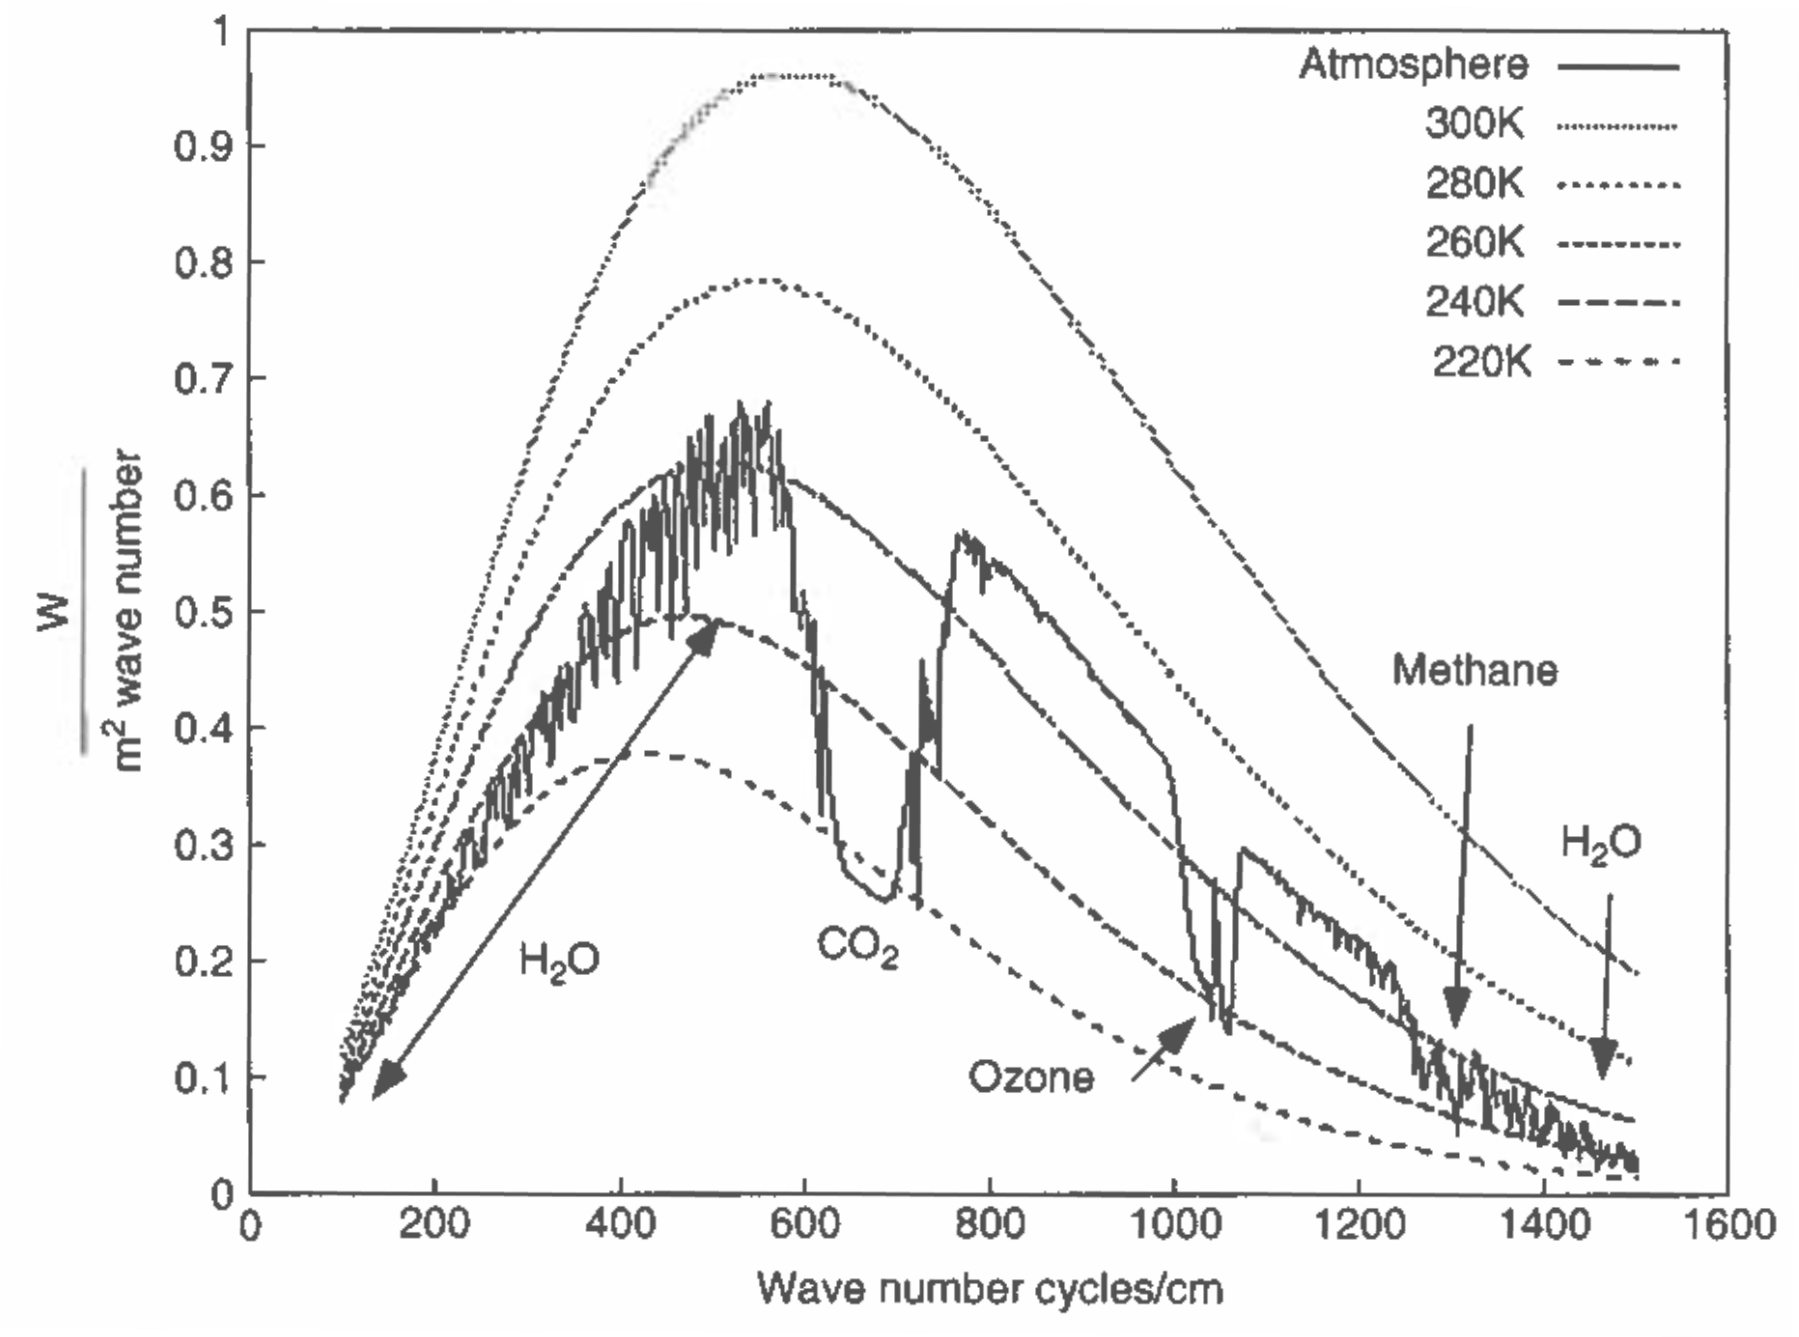
\includegraphics[width=\textwidth]{images/archer_fig-4-3_blackbody-earth.png}\\
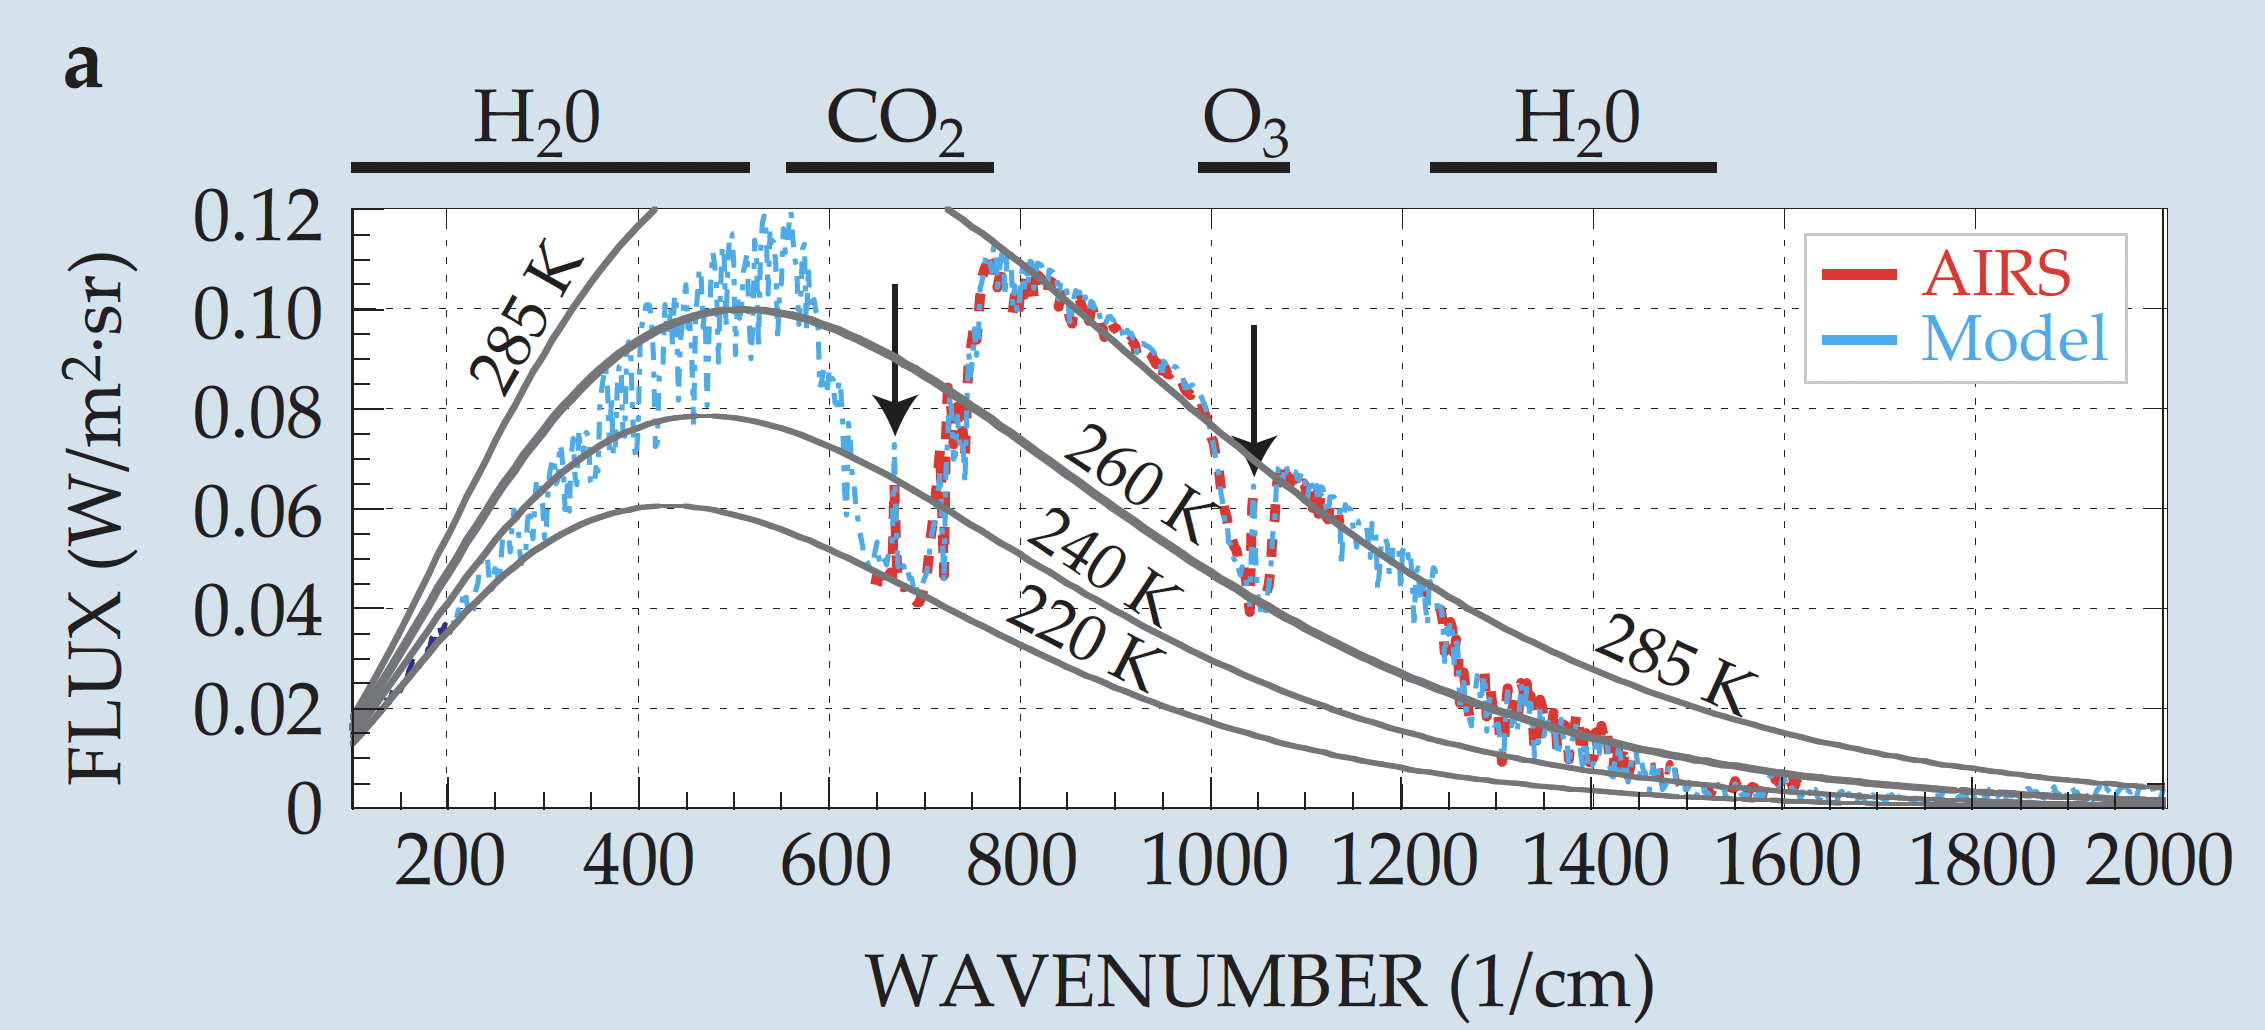
\includegraphics[width=\textwidth]{images/pierrhumbert-physics-today_BB-spectrum-lines-earth_fig3a.png}\\

\caption{ \label{fig:archer-earth-bb}
{\bf Top:} Blackbody curves for different temperatures and a simulated spectrum of Earth as seen from space.  [From Archer's {\em Global Warming: Understanding the Forecast}, Fig 4.3] {\bf Bottom:} Similar graph including actual data from the NASA-AIRS satellite (AIRS) together with model simulated data (Model). [From Pierrehumbert's {\em Physics Today} article (January 2011)]
}
\end{figure}

%%%%%%%%%%%%%%%%%%%%%%%%%%%%%%%%
\newpage

\begin{figure}
\centering
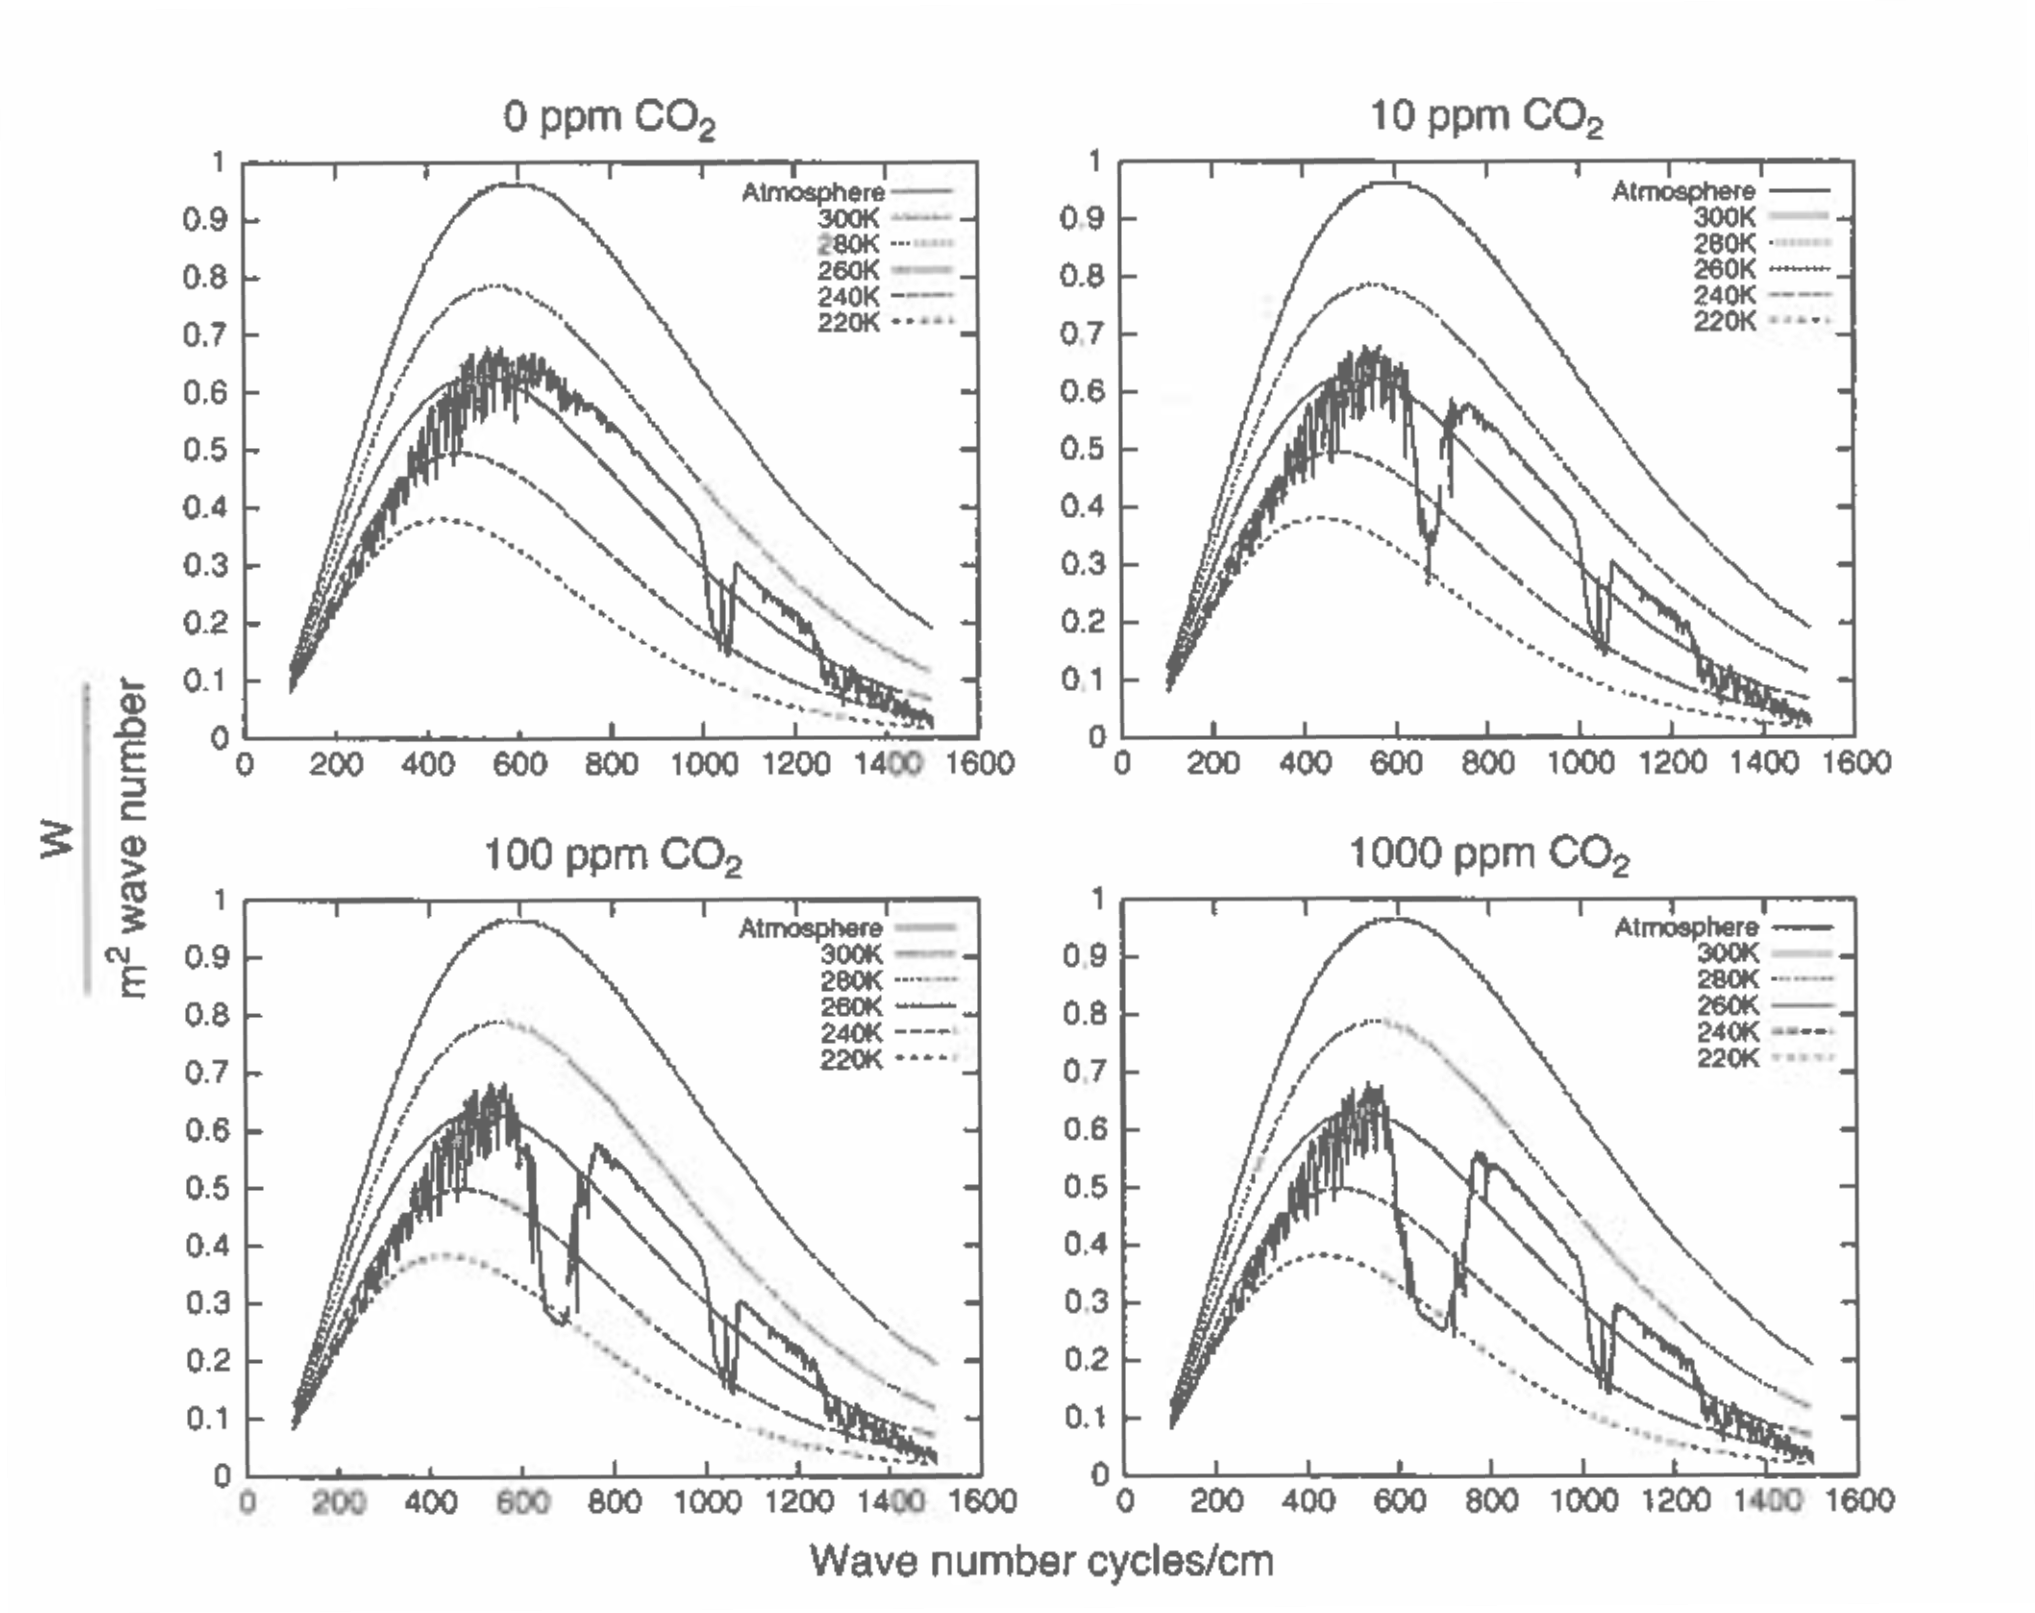
\includegraphics[width=\textwidth]{images/archer_fig-4-5_blackbody-earth-multiple-CO2-concentrations.png}

\caption{  \label{fig:archer-earth-bb-w-diff-CO2}
Blackbody curves for different temperatures and a simulated spectrum of Earth as seen from space, with different simulated amounts of atmospheric carbon dioxide.  [From Archer's {\em Global Warming: Understanding the Forecast}, Fig 4.5]
}
\end{figure}


%%%%%%%%%%%%%%%%%%%%%%%%%%%%%%%%
\newpage

\begin{figure}
\centering
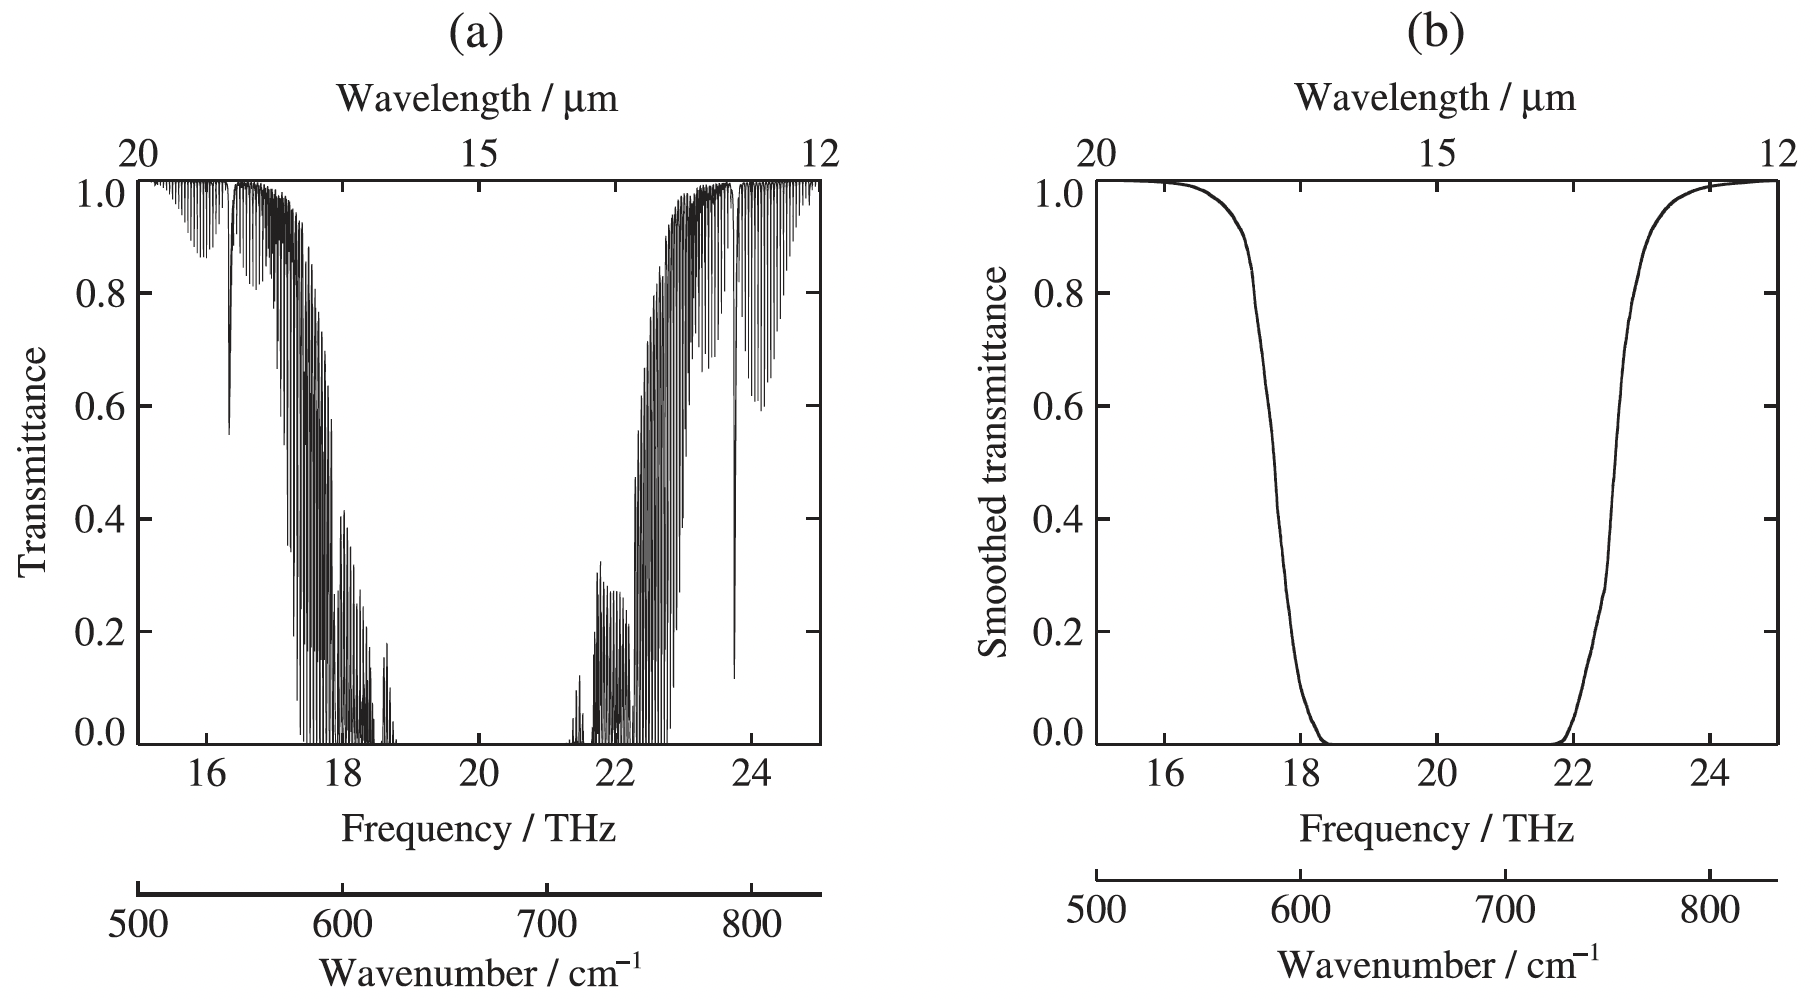
\includegraphics[width=0.65\textwidth]{images/andrews_fig8-5_model-CO2-line-detail-smooth_no-caption.png}\\
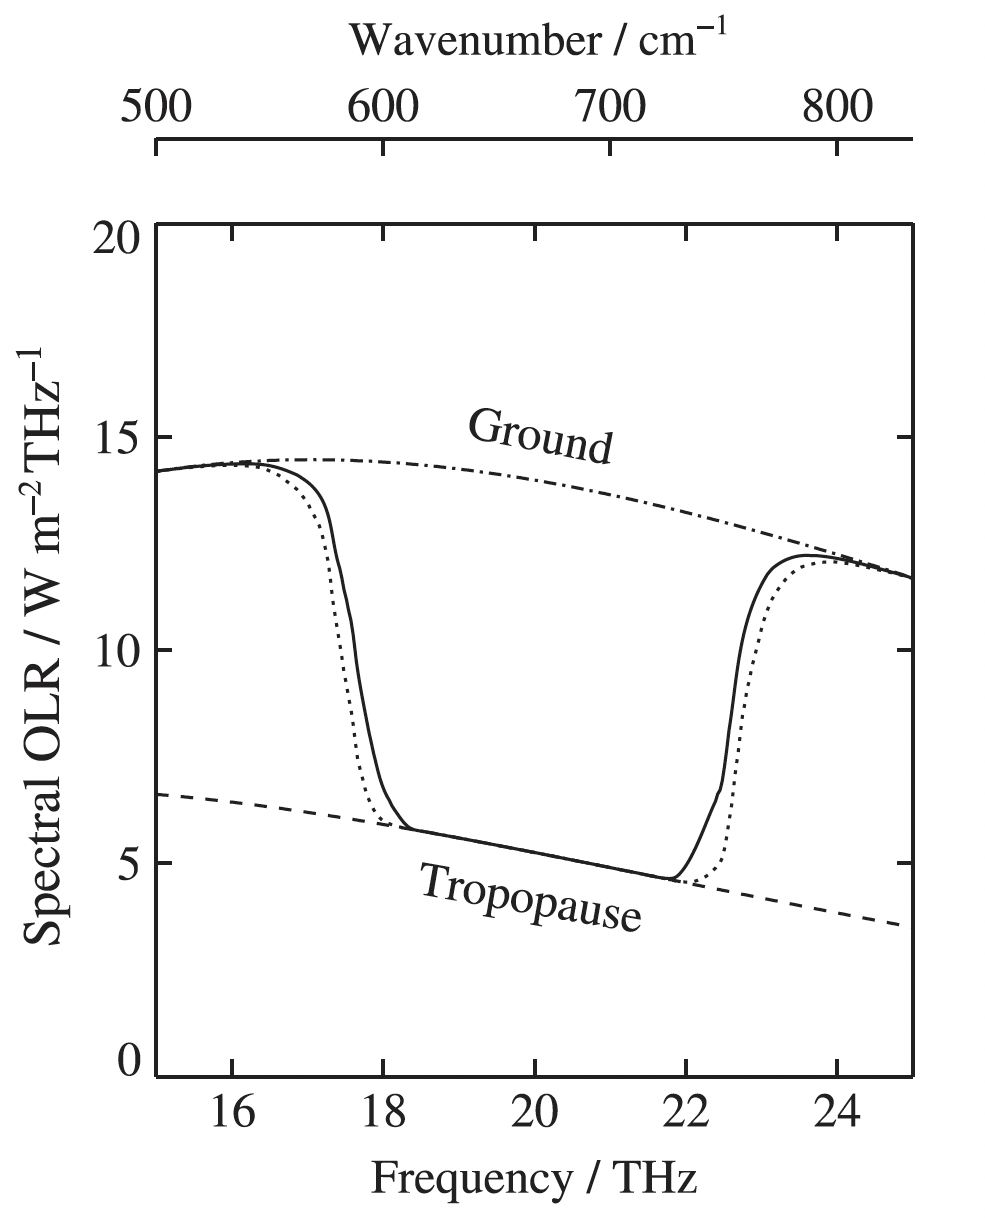
\includegraphics[width=0.7\textwidth]{images/andrews_fig8-7_model-CO2-line-doubled_no-caption.png}

\caption{ \label{fig:andrews-co2-absorption}
{\bf Top:} Absorption spectrum for carbon dioxide, including actual quantum mechanical calculations (left) and smoothed approximation (right). The fine structure seen at left comes from rotational transitions on top of the primary bending transition at \unit{15}{\micro\meter}. [From Andrews' {\em Introduction to Atmospheric Physics} Fig 8.5] {\bf Bottom:} Smoothed carbon dioxide bending transition superimposed on blackbody curve of Earth surface ($T=\unit{290}{\kelvin}$); the blackbody curve of the top of the troposphere is also shown ($T=\unit{225}{\kelvin}$). [From Andrews, Fig 8.7]
}
\end{figure}


%%%%%%%%%%%%%%%%%%%%%%%%%%%%%%%%%%%%%%%%%%%%%%%%%%%%
%%%%%%%%%%                                  References                                %%%%%%%%%%%%%%%%
%%%%%%%%%%%%%%%%%%%%%%%%%%%%%%%%%%%%%%%%%%%%%%%%%%%%
%\noindent {\bf Data Sources}: 



\end{document}
